\section{Investment Universe}
The investment universe is a collection of investable investments for the portfolio management system. The goal is to choose investments with low covariances between each other; hence their combinations can yield better profits from the same risk level\cite{willenbrock2011diversification}. 
\par 
Meir Statman suggested that a well-defined portfolio should have at least 30 or 40 stocks,  \cite{statman1987many}. However, most Exchange Traded Funds (ETFs) combine many investment products and offer investor diversification. Least than ten ETFs are sufficient to produce portfolios with adequate diversification \cite{chang_2016}.
\par
We start from the top 100 ETFs by Asset Under Management (AUM) on March 2021 and remove ones with trading records of less than 14 years. We then obtain the top two most correlated ETFs and remove the one with lower AUM and continue the same process iteratively until 10 ETFs are left (\autoref{appendix:etfs_corr}).
\par
Our selection shows a wide diversity in return and risk, represented in CAGR and stand division of returns.
\begin{figure}[bth]
    \centering
    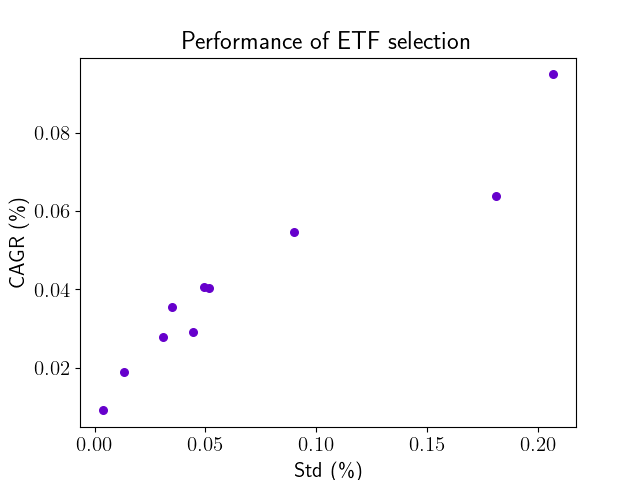
\includegraphics[width=12cm]{images/etfs.png}
    \caption{Performance of ETFs}
    \label{fig:efts}
\end{figure}